%%
%% This is file `sample-sigconf.tex',
%% generated with the docstrip utility,
%% and then modified to 'main.tex' by Dongjun.
%%
%% The original source files were:
%%
%% samples.dtx  (with options: `sigconf')
%% 
%% IMPORTANT NOTICE:
%% 
%% For the copyright see the source file.
%% 
%% Any modified versions of this file must be renamed
%% with new filenames distinct from sample-sigconf.tex.
%% 
%% For distribution of the original source see the terms
%% for copying and modification in the file samples.dtx.
%% 
%% This generated file may be distributed as long as the
%% original source files, as listed above, are part of the
%% same distribution. (The sources need not necessarily be
%% in the same archive or directory.)
%%
%%
%% Commands for TeXCount
%TC:macro \cite [option:text,text]
%TC:macro \citep [option:text,text]
%TC:macro \citet [option:text,text]
%TC:envir table 0 1
%TC:envir table* 0 1
%TC:envir tabular [ignore] word
%TC:envir displaymath 0 word
%TC:envir math 0 word
%TC:envir comment 0 0
%%
%%
%% The first command in your LaTeX source must be the \documentclass command.
\documentclass[sigconf,review,anonymous]{acmart}
\acmConference[ICSE 2022]{The 44th International Conference on Software Engineering}{May 21–29, 2022}{Pittsburgh, PA, USA}

\usepackage{color}
\usepackage{float}
\usepackage{amsmath,amsfonts}
\usepackage[ruled, vlined]{algorithm2e}
\usepackage{graphicx}
\usepackage{textcomp}
\usepackage{xcolor}
\usepackage{listings}
\usepackage{caption}
\usepackage{subcaption}
\usepackage{multirow}
\usepackage{booktabs}
\usepackage{makecell}
\usepackage{galois}
\usepackage{mathpartir}
\usepackage{bussproofs}
\usepackage{mathtools}
\usepackage{colortbl}
\usepackage{hhline}
\usepackage{stmaryrd}
\usepackage{microtype}

% latexdiff
%DIF PREAMBLE EXTENSION ADDED BY LATEXDIFF
%DIF UNDERLINE PREAMBLE %DIF PREAMBLE
\RequirePackage[normalem]{ulem} %DIF PREAMBLE
\RequirePackage{color}\definecolor{RED}{rgb}{1,0,0}\definecolor{BLUE}{rgb}{0,0,1} %DIF PREAMBLE
\providecommand{\DIFadd}[1]{{\protect\color{blue}\uwave{#1}}} %DIF PREAMBLE
\providecommand{\DIFdel}[1]{{\protect\color{red}\sout{#1}}} %DIF PREAMBLE
%DIF SAFE PREAMBLE %DIF PREAMBLE
\providecommand{\DIFaddbegin}{} %DIF PREAMBLE
\providecommand{\DIFaddend}{} %DIF PREAMBLE
\providecommand{\DIFdelbegin}{} %DIF PREAMBLE
\providecommand{\DIFdelend}{} %DIF PREAMBLE
%DIF FLOATSAFE PREAMBLE %DIF PREAMBLE
\providecommand{\DIFaddFL}[1]{\DIFadd{#1}} %DIF PREAMBLE
\providecommand{\DIFdelFL}[1]{\DIFdel{#1}} %DIF PREAMBLE
\providecommand{\DIFaddbeginFL}{} %DIF PREAMBLE
\providecommand{\DIFaddendFL}{} %DIF PREAMBLE
\providecommand{\DIFdelbeginFL}{} %DIF PREAMBLE
\providecommand{\DIFdelendFL}{} %DIF PREAMBLE
%DIF END PREAMBLE EXTENSION ADDED BY LATEXDIFF

% thicker vertical line
\newcolumntype{?}{!{\vrule width 1pt}}

% Styles
\definecolor{dkgreen}{rgb}{0,0.6,0}
\definecolor{gray}{rgb}{0.5,0.5,0.5}
\definecolor{mauve}{rgb}{0.58,0,0.82}
\lstdefinelanguage{JavaScript}{
  keywords={async, await, break, case, catch, class, const, continue, debugger,
    default, delete, do, else, enum, export, extends, false, finally, for,
    function, if, import, in, instanceof, new, null, return, super, switch, this,
    throw, true, try, typeof, var, void, while, with, yield, deref},
  keywordstyle=\color{blue}\bfseries,
  ndkeywordstyle=\color{darkgray}\bfseries,
  identifierstyle=\color{black},
  sensitive=false,
  comment=[l]{//},
  morecomment=[s]{/*}{*/},
  commentstyle=\color{dkgreen}\ttfamily,
  stringstyle=\color{purple}\ttfamily,
  morestring=[b]',
  morestring=[b]"
}
\lstdefinestyle{myJSstyle}{
  language=JavaScript,
  numbers=left,
  stepnumber=1,
  extendedchars=true,
  basicstyle=\footnotesize\ttfamily,
  showstringspaces=false,
  showspaces=false,
  xleftmargin=\parindent,
  tabsize=2,
  breaklines=true,
  showtabs=false,
  captionpos=b
}
\lstdefinestyle{myIR}{
  language=JavaScript,
%  numbers=left,
%  stepnumber=1,
  extendedchars=true,
  basicstyle=\footnotesize\ttfamily,
  showstringspaces=false,
  showspaces=false,
  xleftmargin=\parindent,
  tabsize=2,
  breaklines=true,
  showtabs=false,
  captionpos=b
}
\lstdefinestyle{myDatalog}{
  language=JavaScript,
%  numbers=left,
%  stepnumber=1,
  extendedchars=true,
  basicstyle=\footnotesize\ttfamily,
  showstringspaces=false,
  showspaces=false,
  xleftmargin=\parindent,
  tabsize=2,
  breaklines=true,
  showtabs=false,
  captionpos=b
}
%\lstdefinelanguage{nJavaScript}{
%  keywordstyle=\color{blue}\bfseries,
%  ndkeywordstyle=\color{darkgray}\bfseries,
%  identifierstyle=\color{black},
%  sensitive=false,
%  comment=[l]{//},
%  morecomment=[s]{/*}{*/},
%  commentstyle=\color{dkgreen}\ttfamily,
%  stringstyle=\color{purple}\ttfamily,
%  morestring=[b]',
%  morestring=[b]"
%}
%\lstdefinestyle{nmyJSstyle}{
%  language=nJavaScript,
%  numbers=left,
%  stepnumber=1,
%  extendedchars=true,
%  basicstyle=\footnotesize\ttfamily,
%  showstringspaces=false,
%  showspaces=false,
%  xleftmargin=\parindent,
%  tabsize=2,
%  breaklines=true,
%  showtabs=false,
%  captionpos=b
%}

\lstdefinestyle{common}{
  extendedchars=true,
  basicstyle=\footnotesize\ttfamily,
  showstringspaces=false,
  showspaces=false,
  xleftmargin=\parindent,
  tabsize=2,
  breaklines=true,
  showtabs=false,
  captionpos=b
}

\definecolor{eclipsegreen}{HTML}{008000}
\definecolor{eclipseblue}{HTML}{0000FF}
\definecolor{eclipsegray}{HTML}{808080}
\definecolor{eclipseoperator}{HTML}{8000FF}
\lstdefinestyle{commoncode}{
  style=common,
  keywordstyle=\bfseries\color{eclipseblue},
  commentstyle=\itshape\color{eclipsegreen},
  %identifierstyle=\color{blue},
  stringstyle=\color{eclipsegray},
  numbers=left,
  stepnumber=1,
}
\lstdefinestyle{cpp}{
  style=commoncode,
  language=C++,
  classoffset=1, % starting new class
  %otherkeywords={>,<,.,;,-,!,=,~},
  morekeywords={>,<,.,;,-,!,=,~},
  keywordstyle=\color{eclipseoperator},
  numbers=left,
  stepnumber=1,
}
\lstdefinestyle{codeql}{
  style=commoncode,
  language=C++,
  classoffset=1, % starting new class
  %otherkeywords={>,<,.,;,-,!,=,~},
  morekeywords={>,<,.,;,-,!,=,~,extends},
  keywordstyle=\color{eclipseoperator},
  numbers=left,
  stepnumber=1,
}
\lstdefinestyle{java}{
    style=commoncode,
    language=Java,
}

% Basic
\DeclareMathAlphabet{\mathpzc}{T1}{pzc}{m}{it}
\newcommand{\powerset}[1]{\mathcal{P}(#1)}
\newcommand{\imbox}[1]{\mbox{\small \textit{#1}}}
\newcommand{\name}[1]{\textsf{#1}}
\newcommand{\inred}[1]{{\color{red}{#1}}}
\newcommand{\todo}{\inred{TODO}}
\newcommand{\abs}[1]{{#1}^{\#}}
\newcommand{\finmap}{{\xrightarrow[]{\text{fin}}}}
\newcommand{\mapstos}{\;\dot{\mapsto}\;}
\newcommand{\Dom}{\name{Dom}}

% speed up
\newcommand{\x}{{\textsf{x}}}

% Keywords
\newcommand{\javacode}[1]{\text{\lstinline[style=commoncode,numbers=none]!#1!}}
\newcommand{\ccode}[1]{\text{\lstinline[style=commoncode,numbers=none]!#1!}}
\newcommand{\datalog}[1]{\text{\lstinline[style=myDatalog,numbers=none]!#1!}}
\newcommand{\codeql}[1]{\text{\lstinline[style=commoncode,numbers=none]!#1!}}

% Table 1
\newcommand{\myhead}[3]{
  \multicolumn{1}{c|}{\multirow{2}{*}{\textbf{#1}}} &
  \multicolumn{2}{c|}{\textbf{#2}} &
  \multicolumn{2}{c||}{\textbf{#3}} &
  \multicolumn{1}{c|}{\multirow{2}{*}{\textbf{#1}}} &
  \multicolumn{2}{c|}{\textbf{#2}} &
  \multicolumn{2}{c}{\textbf{#3}}
  %\\\cline{2-5}\cline{7-10}
  \\\hhline{~|----||~|----}
  & \textbf{Lee's~\cite{LeeASE20}} & \textbf{Ours}
  & \textbf{JN-SAF} & \textbf{Ours} &
  & \textbf{Lee's~\cite{LeeASE20}} & \textbf{Ours}
  & \textbf{JN-SAF} & \textbf{Ours}\\\hhline{=|=|=|=|=||=|=|=|=|=}
}
\definecolor{palegreen}{rgb}{0.6, 0.98, 0.6}
\definecolor{pastelgreen}{rgb}{0.47, 0.87, 0.47}
\definecolor{teagreen}{rgb}{0.82, 0.94, 0.75}
\newcommand{\succcolor}{teagreen}

\newcommand{\jnsaf}{JN-SAF\xspace}
\newcommand{\doop}{D\textsc{oop}\xspace}


%%
%% \BibTeX command to typeset BibTeX logo in the docs
\AtBeginDocument{%
  \providecommand\BibTeX{{%
    \normalfont B\kern-0.5em{\scshape i\kern-0.25em b}\kern-0.8em\TeX}}}

%% Rights management information.  This information is sent to you
%% when you complete the rights form.  These commands have SAMPLE
%% values in them; it is your responsibility as an author to replace
%% the commands and values with those provided to you when you
%% complete the rights form.
\setcopyright{acmcopyright}
\copyrightyear{2018}
\acmYear{2018}
\acmDOI{10.1145/1122445.1122456}

%% These commands are for a PROCEEDINGS abstract or paper.
\acmConference[ICSE 2022]{The 44th International Conference on
   Software Engineering}{May 21–29, 2022}{Pittsburgh, PA, USA}
\acmBooktitle{Woodstock '18: ACM Symposium on Neural Gaze Detection,
  June 03--05, 2018, Woodstock, NY}
\acmPrice{15.00}
\acmISBN{978-1-4503-XXXX-X/18/06}


%%
%% Submission ID.
%% Use this when submitting an article to a sponsored event. You'll
%% receive a unique submission ID from the organizers
%% of the event, and this ID should be used as the parameter to this command.
%%\acmSubmissionID{123-A56-BU3}

%%
%% The majority of ACM publications use numbered citations and
%% references.  The command \citestyle{authoryear} switches to the
%% "author year" style.
%%
%% If you are preparing content for an event
%% sponsored by ACM SIGGRAPH, you must use the "author year" style of
%% citations and references.
%% Uncommenting
%% the next command will enable that style.
%%\citestyle{acmauthoryear}

%%
%% end of the preamble, start of the body of the document source.
\begin{document}

%%
%% The "title" command has an optional parameter,
%% allowing the author to define a "short title" to be used in page headers.
\title{Declarative-Style Static Analysis of Multilingual Programs}

%%
%% The "author" command and its associated commands are used to define
%% the authors and their affiliations.
%% Of note is the shared affiliation of the first two authors, and the
%% "authornote" and "authornotemark" commands
%% used to denote shared contribution to the research.
\author{Dongjun Youn}
\authornote{Both authors contributed equally to this research.}
\email{trovato@corporation.com}
\orcid{1234-5678-9012}
\author{Sungho Lee}
\authornotemark[1]
\email{webmaster@marysville-ohio.com}
\affiliation{%
  \institution{Institute for Clarity in Documentation}
  \streetaddress{P.O. Box 1212}
  \city{Dublin}
  \state{Ohio}
  \country{USA}
  \postcode{43017-6221}
}

\author{Joonyoung Park}
\affiliation{%
  \institution{The Th{\o}rv{\"a}ld Group}
  \streetaddress{1 Th{\o}rv{\"a}ld Circle}
  \city{Hekla}
  \country{Iceland}}
\email{larst@affiliation.org}

\author{Sukyoung Ryu}
\affiliation{%
  \institution{Inria Paris-Rocquencourt}
  \city{Rocquencourt}
  \country{France}
}

%%
%% By default, the full list of authors will be used in the page
%% headers. Often, this list is too long, and will overlap
%% other information printed in the page headers. This command allows
%% the author to define a more concise list
%% of authors' names for this purpose.
\renewcommand{\shortauthors}{Trovato and Tobin, et al.}

\abstract[Summary]{
Declarative static program analysis has become one of the widely-used
program analysis techniques thanks to its logical specification:
it specifies ``what'' rather than ``how.''
Declarative static analyzers perform three steps: creating databases of facts from
program source code, evaluating rules to generate new facts, and running queries
over facts to extract all information related to specific properties via
query systems.
Declarative static analyzers can easily support diverse programming languages
as their analysis targets by extending only databases and rules
for new languages. Because query systems are independent of
programming languages, they are reusable for new languages.
However, even when declarative analyzers support multiple
programming languages, they do not support the analysis of multilingual
programs written in two or more programming languages.
With the growing prevalence of multilingual programs in diverse areas,
supporting multilingual program analysis is increasingly important.

In this paper, we propose a systematic methodology that extends a
declarative static analyzer supporting multiple target languages to support
multilingual programs as well. The main idea is to reuse
existing components of the analyzer to minimize the burden of creating new
components.  Our approach first generates a merged database
of facts, consisting of multiple logical language spaces. It allows
existing language-specific rules to derive new facts for the corresponding language
from the facts in the corresponding language space. Then, it defines
language-interoperation rules that handle the language  interoperation semantics.
Finally, it uses the same query system to get analysis results
leveraging the language interoperation semantics.
We develop a proof-of-concept declarative static analyzer for
multilingual programs by extending CodeQL, which can track dataflows
across language boundaries. The analyzer can analyze two types of multilingual programs:
JNI programs written in Java and C, and Python-C programs 
written in Python and C.  We also implement a bug checker on top of
the analyzer to detect dataflow-related interoperation bugs in real-world JNI programs.
Our evaluation shows that the analyzer successfully tracks
dataflows across Java-C and Python-C language boundaries and detects genuine
interoperation bugs in real-world multilingual programs.
}


%%
%% The code below is generated by the tool at http://dl.acm.org/ccs.cfm.
%% Please copy and paste the code instead of the example below.
%%
\begin{CCSXML}
<ccs2012>
 <concept>
  <concept_id>10010520.10010553.10010562</concept_id>
  <concept_desc>Computer systems organization~Embedded systems</concept_desc>
  <concept_significance>500</concept_significance>
 </concept>
 <concept>
  <concept_id>10010520.10010575.10010755</concept_id>
  <concept_desc>Computer systems organization~Redundancy</concept_desc>
  <concept_significance>300</concept_significance>
 </concept>
 <concept>
  <concept_id>10010520.10010553.10010554</concept_id>
  <concept_desc>Computer systems organization~Robotics</concept_desc>
  <concept_significance>100</concept_significance>
 </concept>
 <concept>
  <concept_id>10003033.10003083.10003095</concept_id>
  <concept_desc>Networks~Network reliability</concept_desc>
  <concept_significance>100</concept_significance>
 </concept>
</ccs2012>
\end{CCSXML}

\ccsdesc[500]{Computer systems organization~Embedded systems}
\ccsdesc[300]{Computer systems organization~Redundancy}
\ccsdesc{Computer systems organization~Robotics}
\ccsdesc[100]{Networks~Network reliability}

%%
%% Keywords. The author(s) should pick words that accurately describe
%% the work being presented. Separate the keywords with commas.
\keywords{datasets, neural networks, gaze detection, text tagging}

%%
%% This command processes the author and affiliation and title
%% information and builds the first part of the formatted document.
\maketitle

\section{Introduction}
Declarative static analysis has become one of the widely-used analysis techniques
for detecting bugs and security vulnerabilities in programs.
It specifies ``what'' rather than ``how'' of program analysis and
performs three steps:
1) transforming program source code to a {\it database}
of {\it facts}, 2) generating new facts from known facts by applying
{\it rules}, and 3) extracting information related to specific properties by
applying {\it queries} to the facts via a query system.  DOOP~\cite{doop} is a
declarative static analysis framework conducting points-to analysis for Java
programs. CodeQL~\cite{codeql} is a declarative semantic code analysis engine
maintained by Github, which performs dataflow analysis to detect security
vulnerabilities in Java programs.  Recently, Glean~\cite{glean}, an experimental
declarative query system, has been developed by Meta, on which users can query
information about code structures for JavaScript and Hack programs.

Declarative static analyzers have broadened their analysis targets to diverse
programming languages. To support a new language, one should consider
the three steps of declarative static analysis. Note that because the query
system is independent of analysis target languages, one can reuse the
existing query system for the new language. Therefore, the first step
is to define a new schema of the database containing facts for the new
language and implement a
front-end component that transforms programs written in the new target language into facts.
Then the next step is to define new language-specific rules.  With these
modifications, declarative analyzers can analyze programs written in the new
target language, using the existing queries and the query system.  DOOP currently
supports Python program analysis to detect tensor shape mismatching bugs in
TensorFlow-based Python ML models~\cite{lagouvardos2020static}. CodeQL was
originally designed for Java program analysis, and now it can track dataflows not only
in Java but also in C++, C\#, JavaScript, Ruby, and Python programs.
Furthermore, Glean plans to support diverse target programming languages,
including Python, Java, C++, Rust, and Haskell.

While the analyzers support multiple programming languages, they do not directly
support the analysis of multilingual programs written in two or more
programming languages. Multilingual programs are now widely developed in
various application domains~\cite{kochhar2016large, mergendahlcross}. However,
multilingual programs are often vulnerable to bugs or security issues more than
monolingual programs. A large-scale study on the code quality of multilingual
programs~\cite{kochhar2016large} reported that using multiple languages
together correlates with higher error-proneness. Moreover,
Grichi et al~\cite{grichi2020impact} showed that two or three times more bugs and security
issues had been reported in the language interoperation than in the
intraoperation in widely-used open-source JNI programs such as OpenJ9 and VLC.

In this paper, we propose a systematic methodology that extends a
declarative static analyzer supporting multiple target languages to support
multilingual program analysis as well. Our goal is to maximize the reuse of
already existing components. First, it generates a merged database of facts that can
be separated into multiple logical language spaces.  Each language space
consists of original facts from its corresponding language database, and existing
language-specific rules derive new facts from the facts in the corresponding
language space. Then, to handle the language interoperation semantics in
multilingual programs, we define language-interoperation rules referring to
the language interoperation semantics. The language-interoperation rules derive new
facts from the facts across language spaces. The extensions enable the query system
to extract facts in multilingual programs, taking the language
interoperation semantics into account.
Finally, the same query is evaluated under the same query system to get
analysis results.

To evaluate the practicality of our approach, we develop a proof-of-concept
declarative static analyzer for multilingual programs by extending CodeQL. Our
analyzer tracks dataflows across language boundaries for two types of
multilingual programs: JNI programs written in Java and C and Python-C
programs written in Python and C. The extension is simple enough in that
it requires only a few lines of automated modifications of CodeQL and additional
language-interoperation rules. We also implement a bug checker on top of
the analyzer to detect dataflow-related interoperation bugs in real-world JNI programs.
The evaluation shows that our tool successfully tracks dataflows across
Java-C and Python-C language boundaries and detects genuine interoperation
bugs in real-world multilingual programs.

The contributions of this paper are as follows:
\begin{itemize}
\item We propose a systematic methodology that extends a declarative static analyzer
supporting multiple target languages to support multilingual program analysis.

\item We implement a proof-of-concept declarative static dataflow analyzer for two
types of multilingual programs, Java-C and Python-C, by extending CodeQL.

\item We show the practical usefulness of our analyzer in the sense that it detects
dataflow-related bugs at language boundaries of real-world multilingual
programs.
\end{itemize}

\section{Motivation}

We will introduce a simple/generalized multilingual code example, discuss how
previous works perform analysis for this example, and illustrate some issue for
each approach.

Then, we introduce declarative style analysis, and show how declarative style
dataflow anlysis can be applied.

\subsection{Multilingual program}

Let's look at the following example:

Language A

public void main() \{

  Obj obj = new Obj();

  val = SOURCE;

  SINK = obj.f(val);

\}

Language B

def f(obj: Obj, param: Int): Int \{

  setField(obj, "p", param)

  val ret = getField(obj, "p")

  return ret

\}

What we are interested is whether the data stored in the node named SOURCE can
flow into the node named SINK. For example, SOURCE can be sensitive data like
smartphone's device ID (IMEI), and SINK can be an argument to a logging function.
Another example would be SOURCE being null pointer, and SINK being pointer dereference.

\subsection{Previous approaches for analyzing multilingual program}

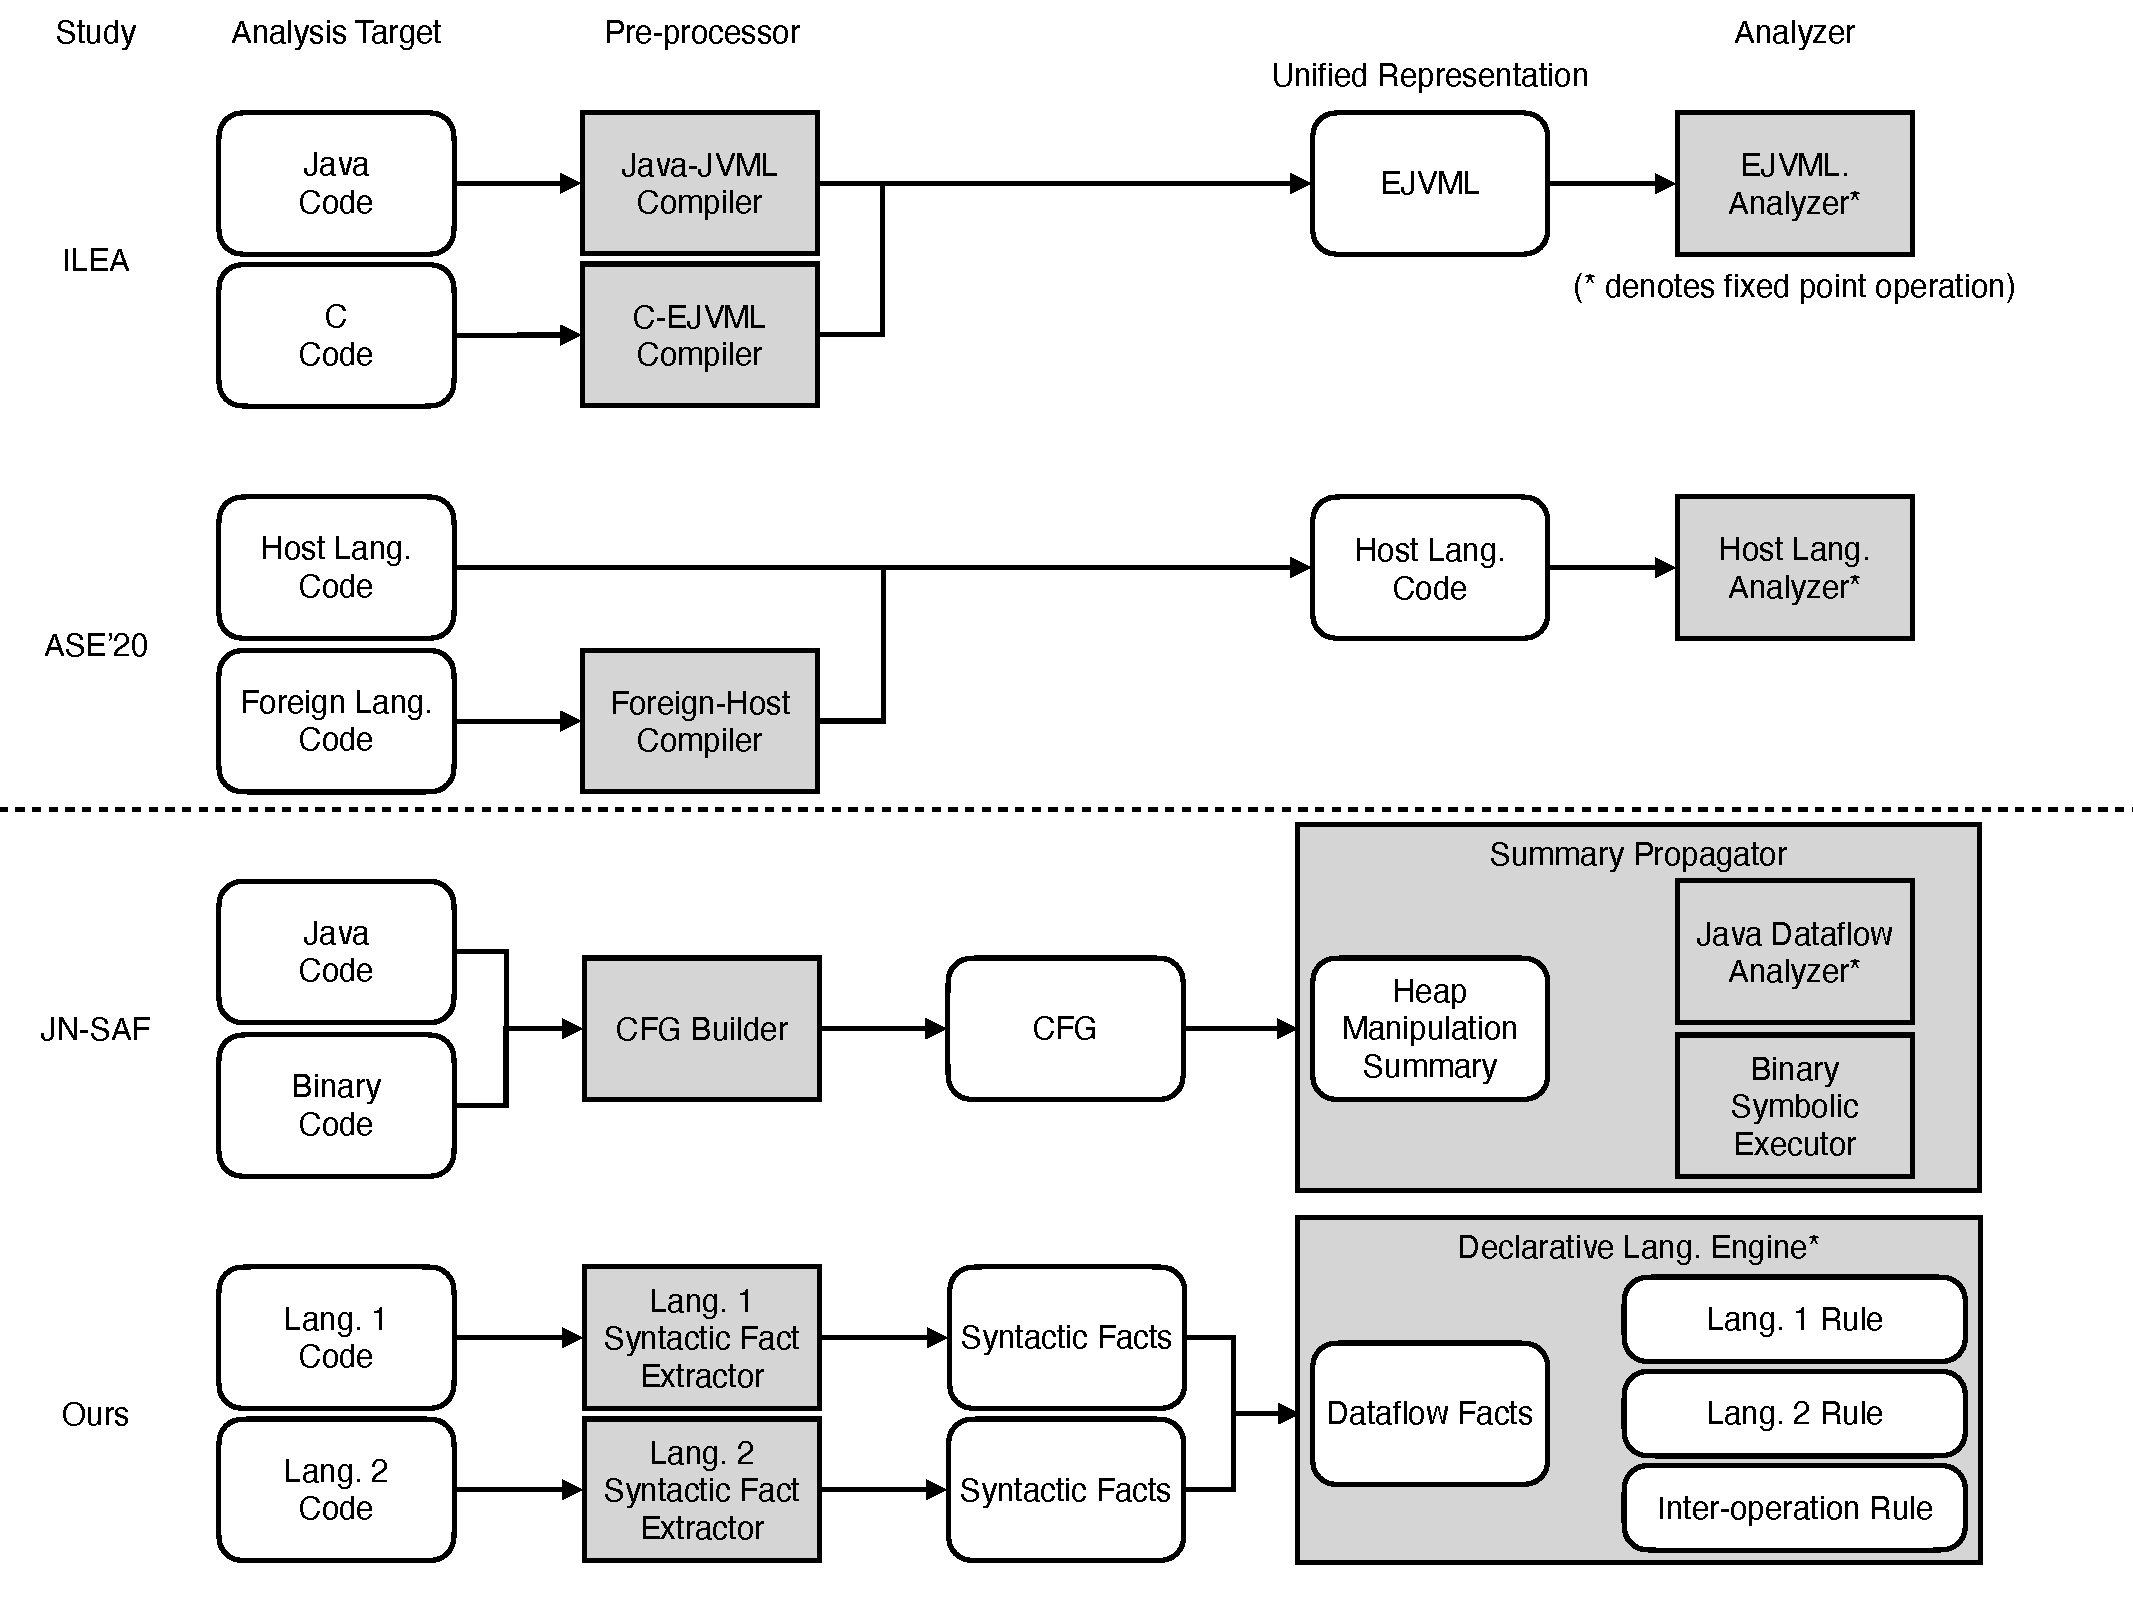
\includegraphics[width=0.5\textwidth]{img/compare}
Fig 0. Approaches for analyzing multolingual programs

There are mainly two approaces for analyzing multilingual programs. One
approach is to define host language and guest language, and transform the guest
language source code into the host language source code. The rationale behind
this approach is that one can resuse the existing analyzers for the host
language source code after the transformation is done.  ILEA[1] is a JNI
program analyzer that adopted this approach. It compiles native C code into
(extended) Java virtual machine language (EJVML), and uses existing analyzer
that works on EJVML, namely Jlint.  Recent study[2] generalizes this idea
and provides formalized method to perform analysis in more general setting.

If we apply this approach to the given example, then the function f of language
B would be compiled into language A as following:

public void f(Obj obj, int param) \{

  obj.p = param;

  int ret = obj.p;

  return ret;

\}

Then, the existing dataflow analyzer can be applied to compile code along with
original code, and would report the dataflow from SOURCE to SINK. The problem
of this approach is that ... (Compile is heavy? Challenging? Not appropriate?
Expressive power of two languaes differ and information is lost when one
language is compield to another?)

Another approach is to use a single framework which incorporates both
languages. JN-SAF[3] is a good example.  JN-SAF is a dataflow analisys tool
specialized for android applications that includes C code as binary.  The core
algorithm it uses is SBDA (summary based dataflow analysis). After constructing
call graph for both Java and native methods, "summary" for each method is
generated for each of methods. Summary is generated in bottom-up manner; if a
method calls another method, the callee method's summary is generated first and
the caller method's summary is generated, possibly using the information from
the callee's summary. (Too long?) This approach solves the problem of
comgpiling languages as previous approach, yet has some limitation in its
implementation detail.
- Symbolic execution -> heavy / slow. - Cycle in call graph -> unsound

\subsection{Declarative style analysis}

In order to solve the problem of JN-SAF, we propose the declarative style
analysis.  The biggest advantage of the declarative style analysis is that
writing analysis in declarative language is simple and light-weight, and it
does not require complex implmentation. For instance, the traditional fix-point
calucation that is used in previous approaches are handled by declarative
language engines, and the programmer for the analyzer does not need to manually
consider such semantics. All they have to write is "declaring" each rules.

For example, we can think of the rule flow(a,b) that will denote the fact that
there is a data flow from node a to node b. This rule can be defined in terms
of another preicate step:

flow(a,b):-step(a,b) or step(a,c) and flow(c,b)

where the predicate step(a,b) denotes the direct data flow from node a and b.
Given the set of facts that denote all the possible dircet steps, then all
possible flow is calculated by evaluating engine. For example, given the facts
that state

step(SOURCE, val)

step(val, param)

step(param, obj.p)

step(obj.p, ret)

step(ret, SINK)

then the declarative language engine can compute the result flow(SOURCE, SINK),
and the analyzer concludes that there is a data flow from SOURCE to SINK.

In the following sections, we formalize the general approach for performing
declartive style dataflow analysis in multilingual program (Section 3), show
the specific implementation of this appraoch for JNI programs, implemented with
CodeQL(Section 4) and show the evaluation result (Section 5).

\section{Modifications}

Modifying the template --- including but not limited to: adjusting
margins, typeface sizes, line spacing, paragraph and list definitions,
and the use of the \verb|\vspace| command to manually adjust the
vertical spacing between elements of your work --- is not allowed.

{\bfseries Your document will be returned to you for revision if
  modifications are discovered.}

\section{Implementation}
In this section, we show how we applied the general idea for multilingual
program analysis into implementing the dataflow analysis tool for JNI programs
using CodeQL, which we named JN-QL. CodeQL is a static analysis engine that
transforms source code into database, and performs analysis by evaluating
"query", written in declarative language called QL (Query langague). In QL,
defining data-facts and rules are referred as defining "predicates", which has
the following form:
\begin{lstlisting}[style=codeql,xleftmargin=2.5em]
predicate isOneTwoThree(int n) {
  n = 1
  or
  n = 2
  or
  n = 3
}
\end{lstlisting}

QL is also object-oriented language, so that it support class definition:
\begin{lstlisting}[style=codeql,xleftmargin=2.5em]
class OneTwoThree extends int {
  OneTwoThree() { // characteristic predicate
    this = 1
    or
    this = 2
    or
    this = 3
  }
}
\end{lstlisting}

Basically, defining class is not really different to defining predicate,
as class is just set of elements that satisfy the predicate called
"characteristic prdicate". For more detailed information about QL, one
refer to the paper[6] or the official document[7].

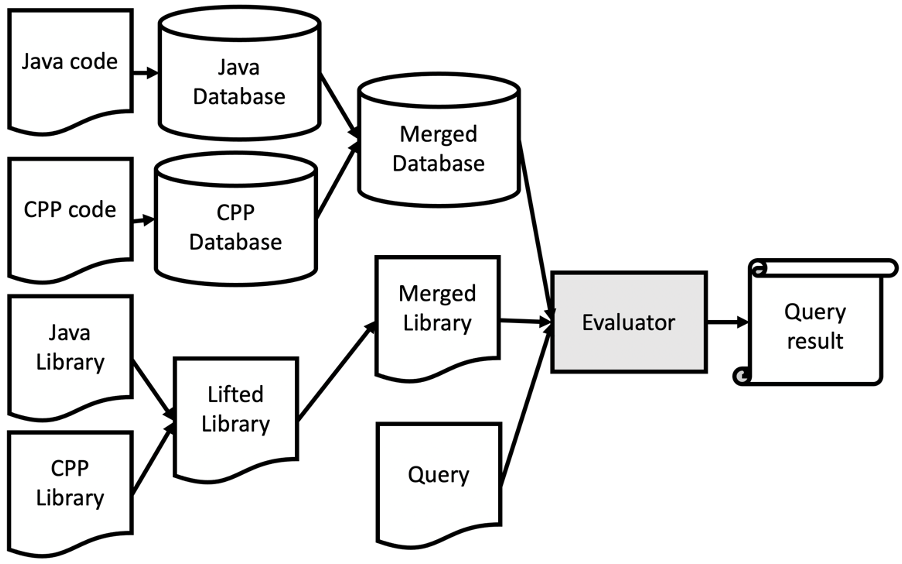
\includegraphics[width=0.5\textwidth]{img/Fig1}
Fig 1.

Figure 1. shows the overall structure of JN-QL. First, it generates database
for each language, C++ and Java, and merge it to one database. This corresponds to a step of
extracting syntactic data-facts from the source code. Then, we merge two
existing dataflow analysis framework, which are part of the library that 
CodeQL provides as a form of library, into one merged library. Finally, using the
merged database and merged library, the user can write a query to perform the
client-analysis, and evaluate it to get analysis result.

\subsection{Create database}
The first step is to gernerate database for each of two languages.  For
compiled languages such as C++ and Java, CodeQL generates database by running
the compiler for each language. While the compiler is running, CodeQL monitors
the behavior of compiler and extracts information it needs, and create database
with that information.  Creation of database for one language is performed in
two steps: first, the extracted information from compiler is stored in the
human readable file format called trap files, and second, these trap files are
then finalized into database, written in binary format.

[Insert example of trap file here]

In order to create a database for two languages, JN-QL performs first step for
each languages separately to get two sets of trap files.  Next step would be to
perfrom finalization step on merged set of trap files. However, a problem is that
both of trap files have table with duplicated name, so simply mering them would not work.
The solution is to add prefix to name of each table. For example, if both
database have tables named "@expr", the table from C++ would be renamed as
"@cpp\_expr", and the table from Java would be renamed as "@java\_expr". After
renaming each table, the second step can be applied to finalize the database on
which the query can be evaluated.

\subsection{Lift library}
CodeQL provides various libraries for each languages, which consists of some
pre-defined predicates and classes that can be useful for user to implement
analysis on their own taste. Dataflow analysis library is one of them, and both
C++ and Java supports this dataflow anslysis library. Two dataflow analysis
library have same framework: they share same classes such as "Node", and some
predicates such as "simpleLocalFlowStep".

\begin{lstlisting}[style=codeql,xleftmargin=2.5em]
class Node extends TNode {
  ...
}
predicate simpleLocalFlowStep(Node nodeFrom, Node nodeTo) {
  // Expr -> Expr
  exprToExprStep_nocfg(
    nodeFrom.asExpr(),
    nodeTo.asExpr()
  )
  or
  // Assignment -> LValue post-update node
  ...
}
//cpp/dataflow/internal/DataFlowUtil.qll
class Node extends TNode {
  ...
}
predicate simpleLocalFlowStep(Node node1, Node node2) {
  // Variable flow steps through
  // adjacent def-use and use-use pairs.
  exists(SsaExplicitUpdate upd |
    upd.getDefiningExpr().(VariableAssign).getSource()
    = node1.asExpr() or
    upd.getDefiningExpr().(AssignOp) = node1.asExpr()
  |
    node2.asExpr() = upd.getAFirstUse()
  )
  or
  // Flow through this
  ...
}
//cpp/dataflow/internal/DataFlowUtil.qll
\end{lstlisting}
However, these two implementations are not compatible, that is, although they have the same name,
we can not use "Node" class of C++ as an argument for "simpleLocalFlowStep" predicate of Java or vice versa.
Therefore, we lift each of the library into the same level so that classes and predicates become compatible.
First, we encapsulated each of original dataflow into CodeQL's module, named CPP and JAVA so that
original classes and predicated can be distinguished with lifted ones.
A class can be lifted by first defining sum type, which denotes that the lifted class would be either from C++ or
Java, and then make the lifted class be of that type. We also implemented two member predicates that can cast
the lifted class into each of corresponding class.
\begin{lstlisting}[style=codeql,xleftmargin=2.5em]
private newtype TNode =
  TJavaNode(JAVA::Node n)
  or
  TCppNode(CPP::Node n)
class Node extends TNode {
  JAVA::Node asJavaNode() {
    this = TJavaNode(result)
  }
  CPP::Node asCppNode() {
    this = TCppNode(result)
  }
  ...
}
\end{lstlisting}

A predicate can be lifted by combining two original predicates with "or" connectives.
For each original predicate, each of the arguments and return values are casted down to
correspnding language's class. After lifting, the lifted predicate shows equlivalent behavior
as the original ones if all the arguments are from the same language.
\begin{lstlisting}[style=codeql,xleftmargin=2.5em]
predicate simpleLocalFlowStep(Node node1, Node node2) {
  JAVA::simpleLocalFlowStep(
    node1.asJavaNode(), node2.asJavaNode()
  )
  or
  CPP::simpleLocalFlowStep(
    node1.asCppNode(), node2.asCppNode()
  )
}
\end{lstlisting}
\subsection{Merge library}

After the library is lifted, the last step is to extend some predicates to reflect the
semantics of interoperation between languages. For example, the predicate named "viableCallable"
is a predicate for connecting function call and target function. It gets argument of class "DataFlowCall",
and the result is of class "DataFlowCallable". After merging the libraries, this predicate would be as follow:

\begin{lstlisting}[style=codeql,xleftmargin=2.5em]
DataFlowCallable viableCallable(DataFlowCall c) {
result.asJavaDataFlowCallable()
  = JAVA::viableCallable(c.asJavaDataFlowCall()) or
result.asCppDataFlowCallable()
  = CPP::viableCallable(c.asCppDataFlowCall()) or
result.asCppDataFlowCallable()
  = viableCallableJ2C(c.asJavaDataFlowCall()) or
result.asJavaDataFlowCallable()
  = viableCallableC2J(c.asCppDataFlowCall())
}
\end{lstlisting}

The first two lines are result of lifting, and they take advantage of the
original predicates from dataflow library.  They handle the call edges from
Java to Java, and from C++ to C++.

Next two lines are the result of merging library, and they are responsible for
inter-language call edges.  The predicate "viableCallableJ2C" finds call edges
from Java to C++, and the predicate "viableCallableC2J" finds call edges from
C++ to Java. One thing to note here is that, function call from Java to C++
and function call from C++ to Java is different. Function call from Java to C++
is mostly static, that is, the target of function call can be determined in compile
time, without requiring run-time value. On the other hand, the method call from C++
to java requires runtime value. The method call from C++ to java is done by calling
interface function: callJavaMethod(name, args...). The target
method's name is passed as a string value to the argument "name",
and in order to determine correct function call target, the value stored in the argument
should be identified. In order to correctly analyze this feature, we used "inner-flow"
to determine what string values can flow into this argument.

\subsection{JNI specific details}
\inred{Write JNI-specific implementation details here: method, class as node / identify jni call / reduce time?}

\section{Evaluation}
In this section, we show the feasibility of the approach of using declarative
analysis for multilingual program, and the effectiveness of its
implentation. More specifically, we set three research questions as follow:

RQ1) Feasibility: Is it possible to implement a working static analyzer for multilingual program in declarative style?

RQ2) Performance: How is the spped and precision of implemented analyzer, compared to the state-of-the-art analyzer?

RQ3) Usefulness: How practical is the implemented analyzer?

To answer RQ1, we ran our implemented analyzer to NativeFlowBench, which is a
small set of becnhmarks manually crafted by authors of JN-SAF[2], with the
purpose of testing dataflow analyzer for JNI programs. It consists of 23
android applications featuring various interactions between C++ and Java, some
of which contain a malicious code pattern that tries leak sensitive user data.
To answer RQ2, we ran our analyzer to 42 real-world android applications
collected from F-Droid[9], a repository for open-source android application. These
42 apps are selected by searching for apps with JNI, and among them, selecting those
that we could sucessfully compile. We compared our analyzer with
state-of-the-art[3] JNI analyzer, and confirmed that our analyzer outperforms
in terms of scalability and precision.  To answer RQ3, we implemented various
kinds of bug checkers, illustrated in previous researches[1][3], on top of our
analyzer. We ran our bug checker on the 42 applications of F-Droid mentioned
above, and discovered 38 bugs, including 30 newly found bugs.


\subsection{RQ1: Feasibility}
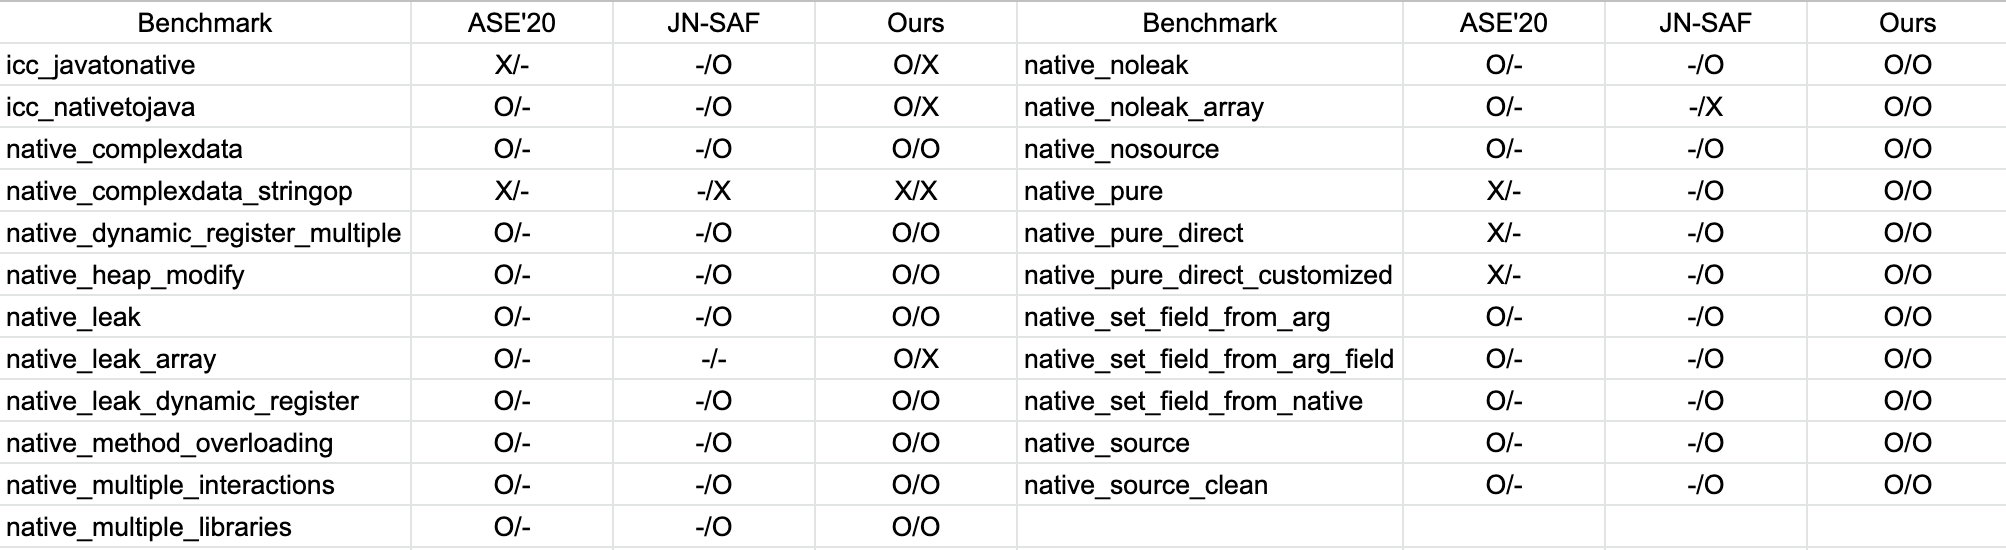
\includegraphics[width=0.5\textwidth]{img/table1}
The table1 shows the analysis result for 19 benchmarks in NativeFlowBench.  The
"Benchmark" coulmns denote the benchmark names, and "result" coulmns denote
whether the analysis result for corresponding benchmark was correct(O) or
not(X). We call that the analysis result is successful if every function call
target (call(j->c), call(c->j)) and field access tagret (field\_read(c->j),
field\_write(c->j)) are precisely determined, and every data leak is reported
correctly without false positives or false negatives.  The result shows that
except for one benchmark, our analyzer could correctly determine all targets
for function calls and field access correctly, and could successfully perform
dataflow analysis to find all of the data leaks. The only exception was
native\_compexdata\_stringop, where string manipulation functions such as
strcpy or strcat from C++'s standard library were used to create the string
value that indicates the target method's name, and since the inner-flow
analysis could not properly handle these functions, analyzer could not
correctly deterimine the function call target.

(Emphasize that data leak was not found in the previous research? or not?)

\subsection{RQ2: Performance}
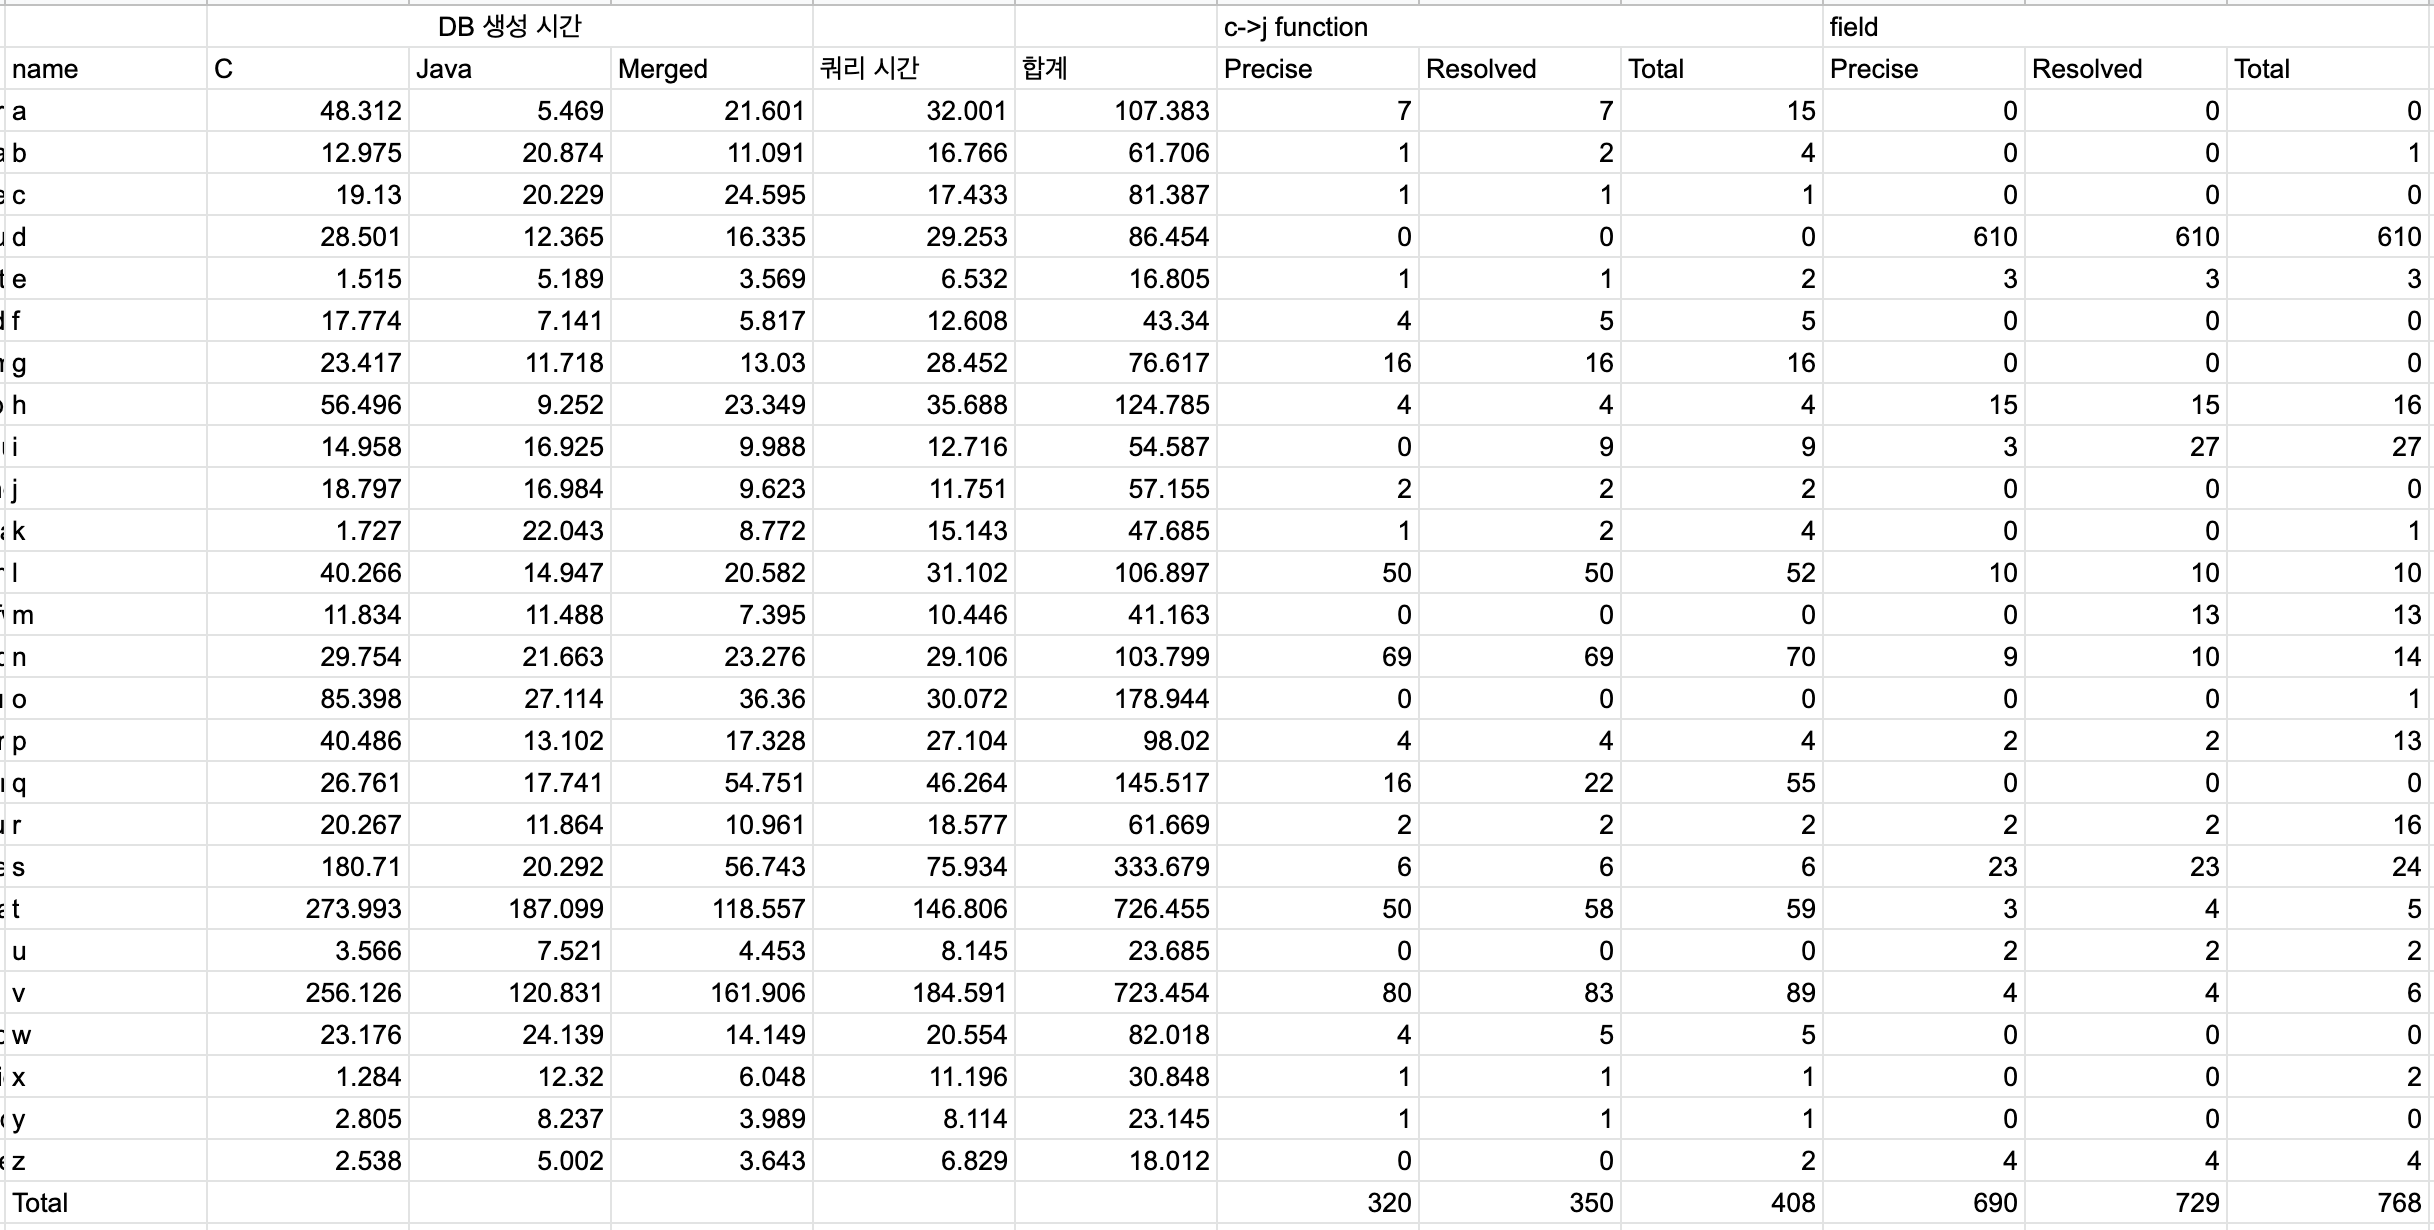
\includegraphics[width=0.5\textwidth]{img/table2}
The table2 shows the analysis result for 42 F-Droid applications. The "time"
coulmn denotes the time for creating database and evaluating query. The average
time for creating DB was ??? seconds, and average time for evaluating query was
??? seconds, making the total analysis time ??? seconds. This is x4 faster on
average, compared to the state-of-the art JNI program analyzer.  Note that time
for creating DB includes compile time, and once DB is created, multiple queries
can be evaluated withou creating DB again. This means that pratically, the
pratical speed up becomes x14.

The "precision" coulms denotes the precision of dispatching function call
target, and field access target.  "Precise" means exactly one target was found,
and resolved means at least one target was found.  Compared to the previous
result, the precision was also higher for both function call targets and field
access targets.

\subsection{RQ3: Usefulness}


\section{Related Work}\label{sec:related}
For Java-C program analysis, ILEA~\cite{ILEA} extends
the Java Virtual Machine Language (JVML) and Jlint, a dataflow analyzer for
Java bytecode, to compile both Java and C code to the extended JVML and analyze
the integrated programs.  Since the modest extension of JVML cannot
support the full C semantics like the C memory model, it extremely over-approximates C
operations such as reads and writes through pointers.  Lee et al.~\cite{LeeASE20}
proposed a general approach to analyzing multilingual programs written in both
{\it host} and {\it guest} languages.  Their approach first uses a guest
language analyzer to extract semantics summaries from the parts written in the
guest language, C in their implementation, translates and integrates the
summaries into a host language, Java, and then performs the whole-program
analysis using a host language analyzer. 
%While their approach leverages the
%full features of existing static analyzers, \ours inherits the query-based
%analysis and can compute target properties effectively without expensive and
%redundant computation.

Researchers also studied binaries rather than C/C++ source code
for Java-C program analysis. Fourtounis et al.~\cite{scanning} proposed a lightweight reverse engineering technique to
recover Java method calls from binaries instead of performing heavy analyses on
binary code.  Their reverse engineering generates datafacts of Java method
calls from binaries, which can be used in further declarative-style Java
analyses. While the approach is lightweight but targets only Java method call
identification in binaries, our approach seamlessly analyzes dataflows across language
boundaries between Java and C.  JN-SAF~\cite{JN-SAF} defines a
unified dataflow summary to represent dataflows in both Java bytecode and
binary.  It extracts summaries from each Java method with a Java static
analyzer and from each native function with a binary symbolic execution, and
composes the summaries in a bottom-up manner to find data leakages over
language boundaries.
%It sacrifices the performance to analyze every possible
%dataflow from binaries using the expensive symbolic execution. On the contrary, our
%approach is scalable in that the query-based approach analyzes only necessary
%dataflows when C source code is available.

Android hybrid apps are
written in both Java and JavaScript, taking advantage of the portability from
JavaScript and device resource accessibility from Java.
HybriDroid~\cite{hybridroid}, implemented on top of WALA~\cite{WALA}, analyzes
Java and JavaScript code seamlessly to detect programmer errors on
interoperations and track data leakages across language boundaries.
Bae et al.~\cite{BaeICSE19} tackled the expensive analysis of HybriDroid and proposed
a lightweight type system detecting the same kinds of programmer errors in
Android hybrid apps. Jin et al.~\cite{jin2014code} proposed static detection
of code injection attacks from JavaScript to Java.  They manually
modeled Java frameworks and performed a taint analysis for JavaScript with the models.


Python supports an interoperability mechanism with C~\cite{PythonC}.
Developers often import performance-critical C code to high-level Python code.
Recent work~\cite{sas2021} proposed a Python-C analyzer by reusing existing
Python and C analyzers built on top of the same framework, MOPSA~\cite{Mopsa}.
They leverage the full features of the analyzers within the same framework to
perform precise context-sensitive value analyses. 
\inred{Polycruise~\cite{polycruise} is a Python-C analyzer that enables an efficeint
dynamic information flow analysis(DIFA).
(...)
In contrast to these works}, our work focuses on declarative style dataflow analysis. 

\section{Conclusion}\label{sec:conclude}
Declarative static analysis has become a widely-used analysis technique but has
not supported multilingual programs actively developed in diverse application
domains.  In this paper, we present a practical extension methodology for a
declarative static analyzer that supports multiple languages to analyze
multilingual programs.  The first step is to create a merged database
consisting of multiple logical language spaces. Each language space stores
facts transformed from source code written in its corresponding language.
Then, the second step is to define language-interoperation rules to derive
facts across language boundaries.  Our prototype implementation, \ours built on
top of CodeQL, successfully tracks dataflows over language boundaries in both
Java-C and Python-C programs.  Using \ours, we found 33 true bugs and
vulnerabilities from real-world JNI applications, 12 of which are from the
applications that \lees, the state-of-the-art Java-C program analyzer, failed
to analyze due to the lack of scalability.  We believe that our approach is
applicable to various multilingual programs, beyond Java-C and Python-C, and to
multiple types of analyses.


%%
%% The acknowledgments section is defined using the "acks" environment
%% (and NOT an unnumbered section). This ensures the proper
%% identification of the section in the article metadata, and the
%% consistent spelling of the heading.
\begin{acks}
ACK. SYN. SYNACK.
\end{acks}

%%
%% The next two lines define the bibliography style to be used, and
%% the bibliography file.
\bibliographystyle{ACM-Reference-Format}
\bibliography{ref}

\end{document}
\endinput
%%
%% End of file `main.tex'.
